\appendix

\section{Supplementary Figures and Tables}

This appendix provides additional spatial, temporal, and sensitivity analysis figures referenced in the main text. These materials offer detailed visual evidence supporting the manuscript's findings on deforestation patterns, regional heterogeneity, and optimal forest management trajectories.

\subsection{Temporal and Emissions Analysis}

\begin{figure}[H]
    \centering
    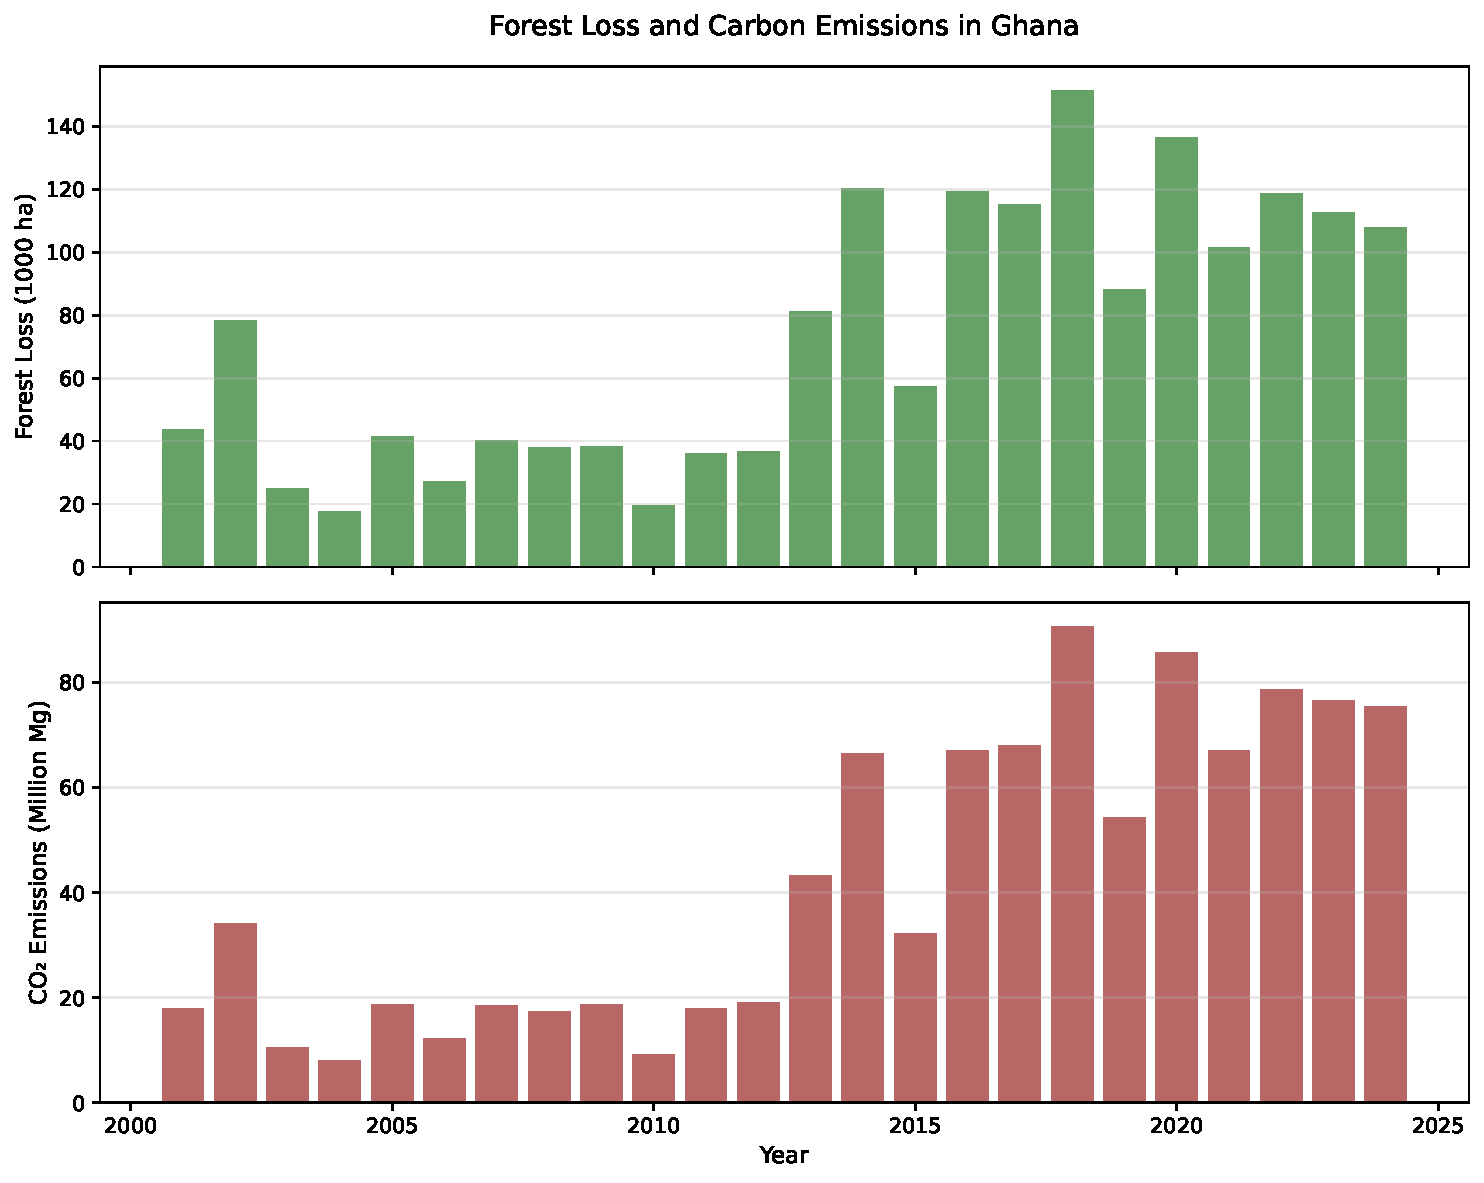
\includegraphics[width=0.9\textwidth]{figures/fig2_emissions.pdf}
    \caption{Cumulative Carbon Emissions from Tree Cover Loss (2001-2024). Total emissions reached 487 million Mg CO$_2$e over the 24-year period. The acceleration in emissions post-2016 corresponds to the recent deforestation surge, with annual emissions increasing from 16 million Mg CO$_2$e (2007-2015 average) to 24 million Mg CO$_2$e (2016-2024 average). This 50\% increase in emission intensity reflects both higher clearing rates and targeting of primary forests with greater carbon stocks.}
    \label{fig:emissions}
\end{figure}

\begin{figure}[H]
    \centering
    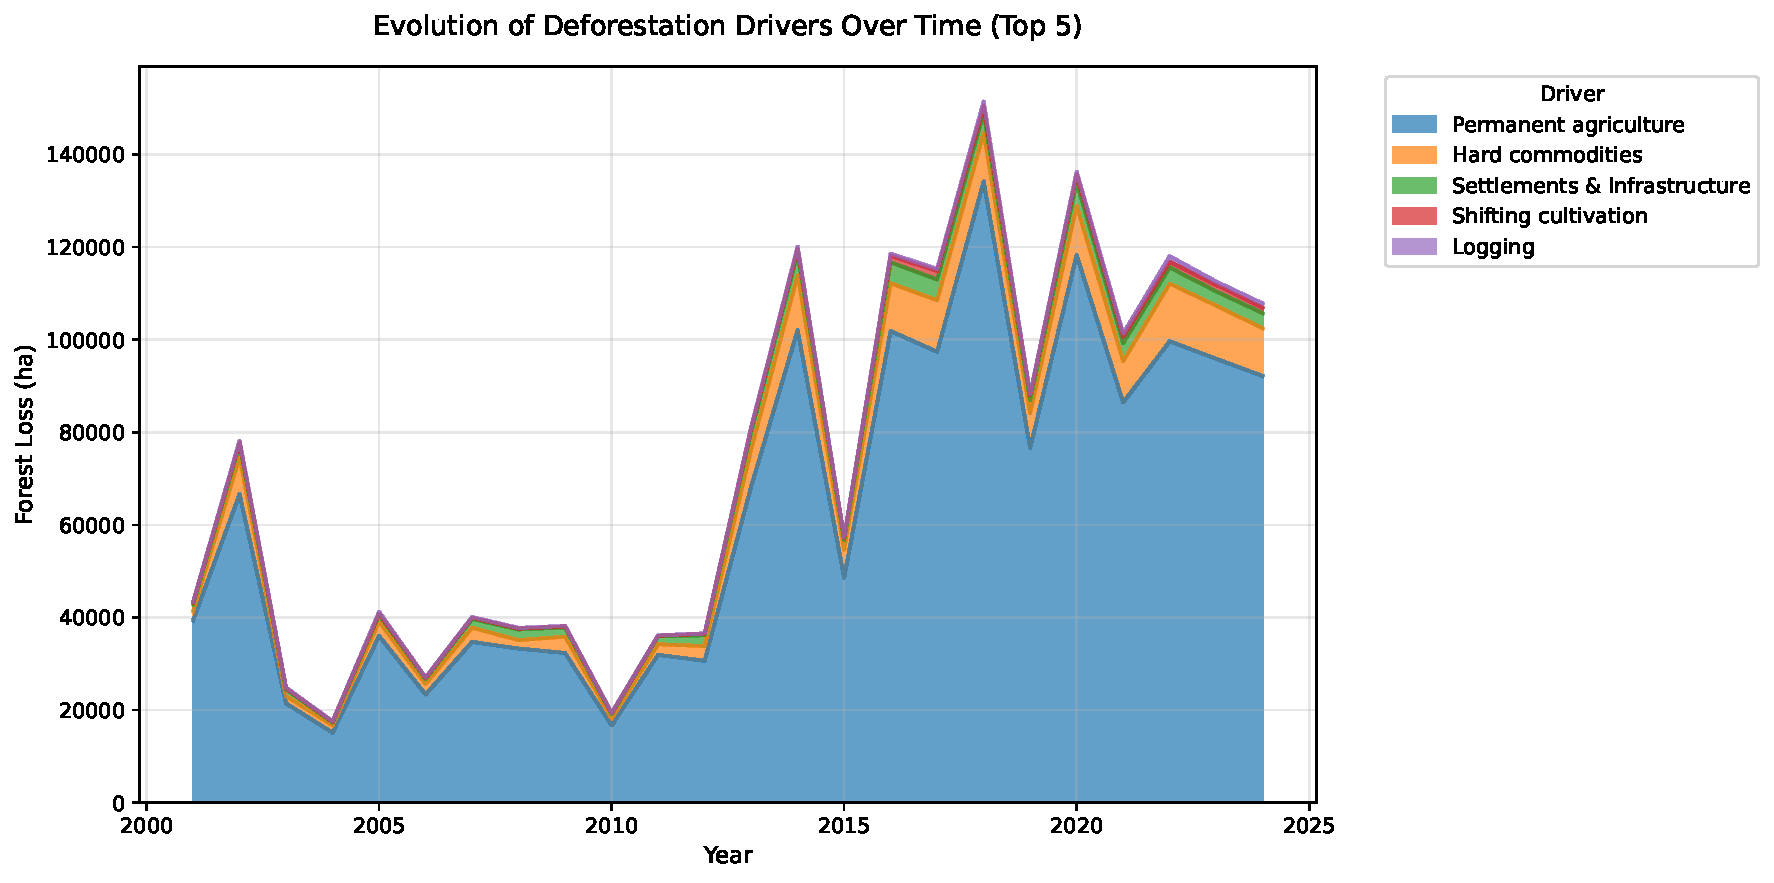
\includegraphics[width=0.9\textwidth]{figures/fig4_drivers_time.pdf}
    \caption{Evolution of Deforestation Drivers Over Time (2001-2024). Commodity agriculture's share increased from 84\% in 2001-2005 to 93\% in 2020-2024, while shifting cultivation declined from 9\% to 3\%. This transition reflects agricultural commercialization—smallholders abandoning traditional forest-fallow systems for permanent cocoa cultivation. Forestry operations remain relatively stable at 3-4\%, while urbanization pressures gradually increase from 0.8\% to 1.8\%, concentrated near Accra and Kumasi metropolitan areas.}
    \label{fig:drivers_time}
\end{figure}

\begin{figure}[H]
    \centering
    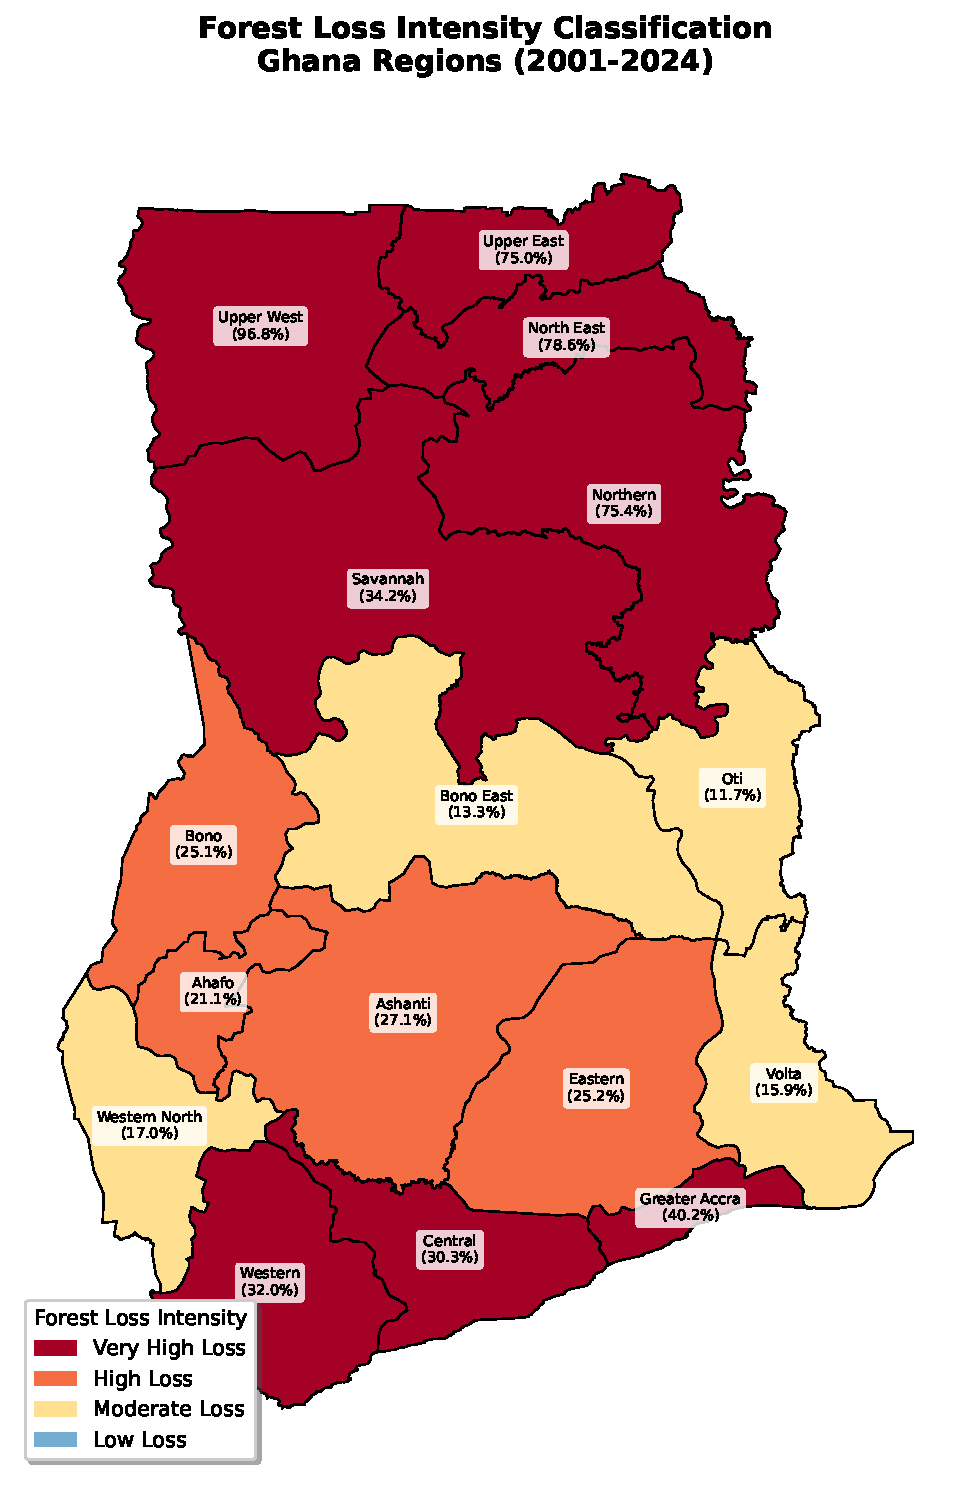
\includegraphics[width=0.9\textwidth]{figures/fig15_loss_categories.pdf}
    \caption{Tree Cover Loss Categories: Primary Forest, Natural Forest, and Total Loss. Primary forest loss (darker green line) accounts for 42\% of total deforestation, disproportionately contributing to biodiversity loss and carbon emissions given higher biomass density. The divergence between primary and total forest loss after 2015 indicates increasing pressure on previously intact forests, suggesting enforcement weakening in protected zones where primary forests concentrate.}
    \label{fig:loss_categories}
\end{figure}

\subsection{Regional Trends and Spatial Patterns}

\begin{figure}[H]
    \centering
    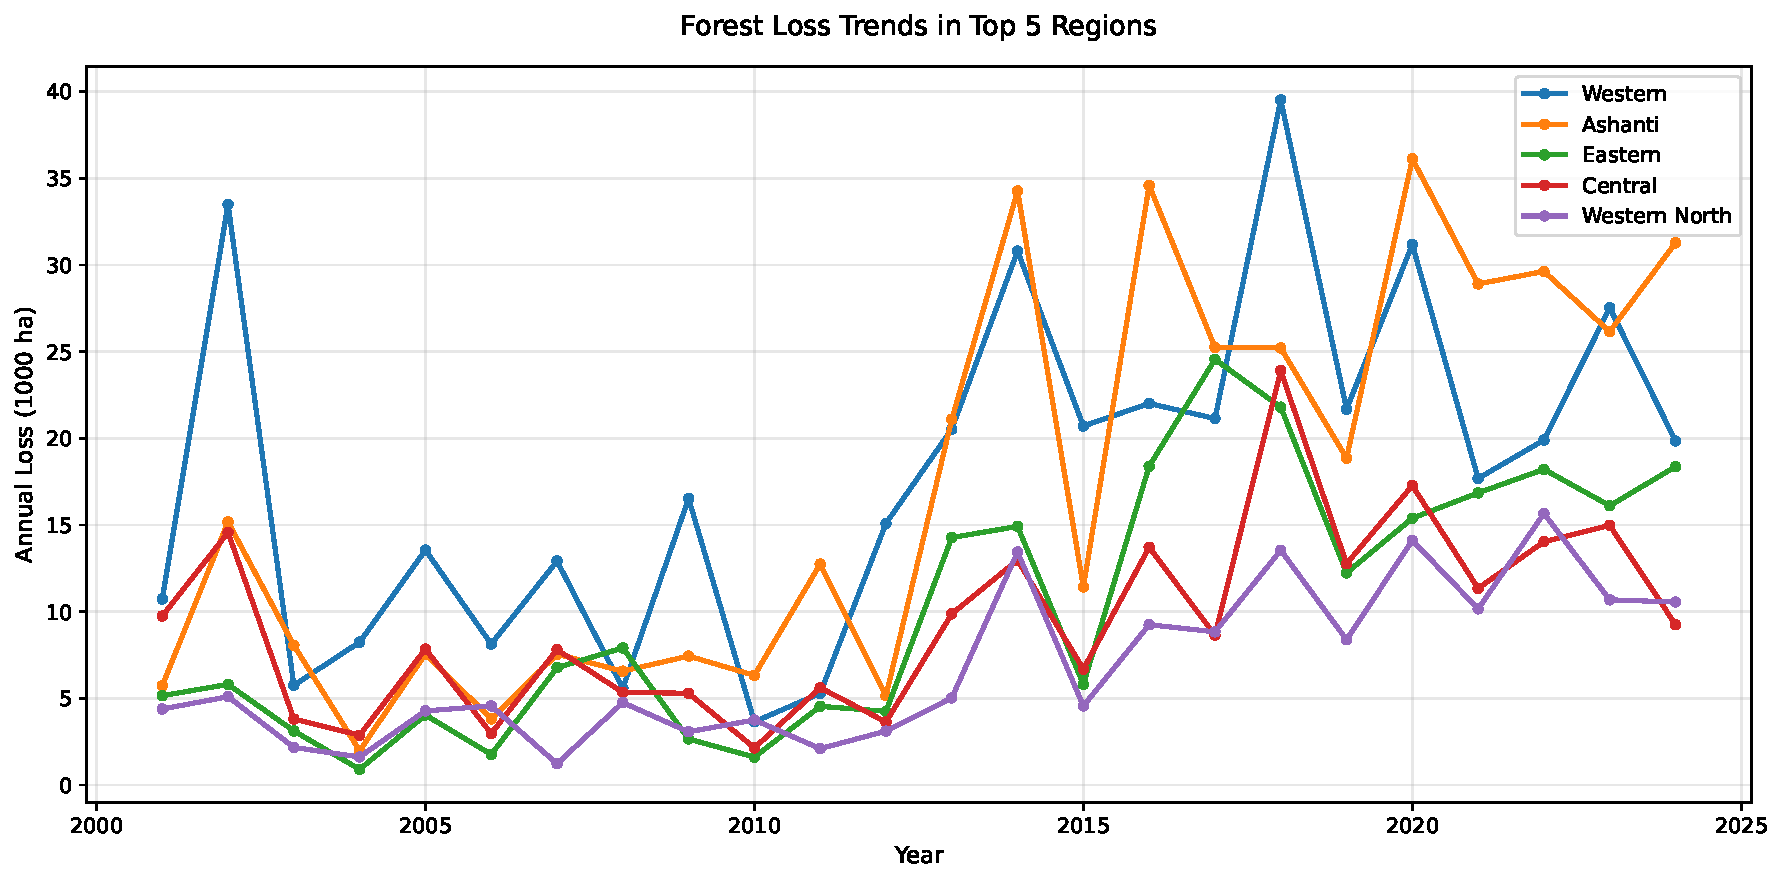
\includegraphics[width=0.95\textwidth]{figures/fig6_regional_trends.pdf}
    \caption{Regional Deforestation Trends Over Time (2001-2024). Eastern and Ashanti regions show consistently high loss rates throughout the period, averaging 13,000 ha/year and 11,000 ha/year respectively. Western region exhibits more volatility, with peaks in 2002 (22,000 ha) and 2020 (18,000 ha) corresponding to cocoa price spikes. Northern regions maintain low, stable loss rates below 2,000 ha/year. The lack of convergence across regions suggests spatially heterogeneous drivers requiring differentiated policy responses.}
    \label{fig:regional_trends}
\end{figure}

\begin{figure}[H]
    \centering
    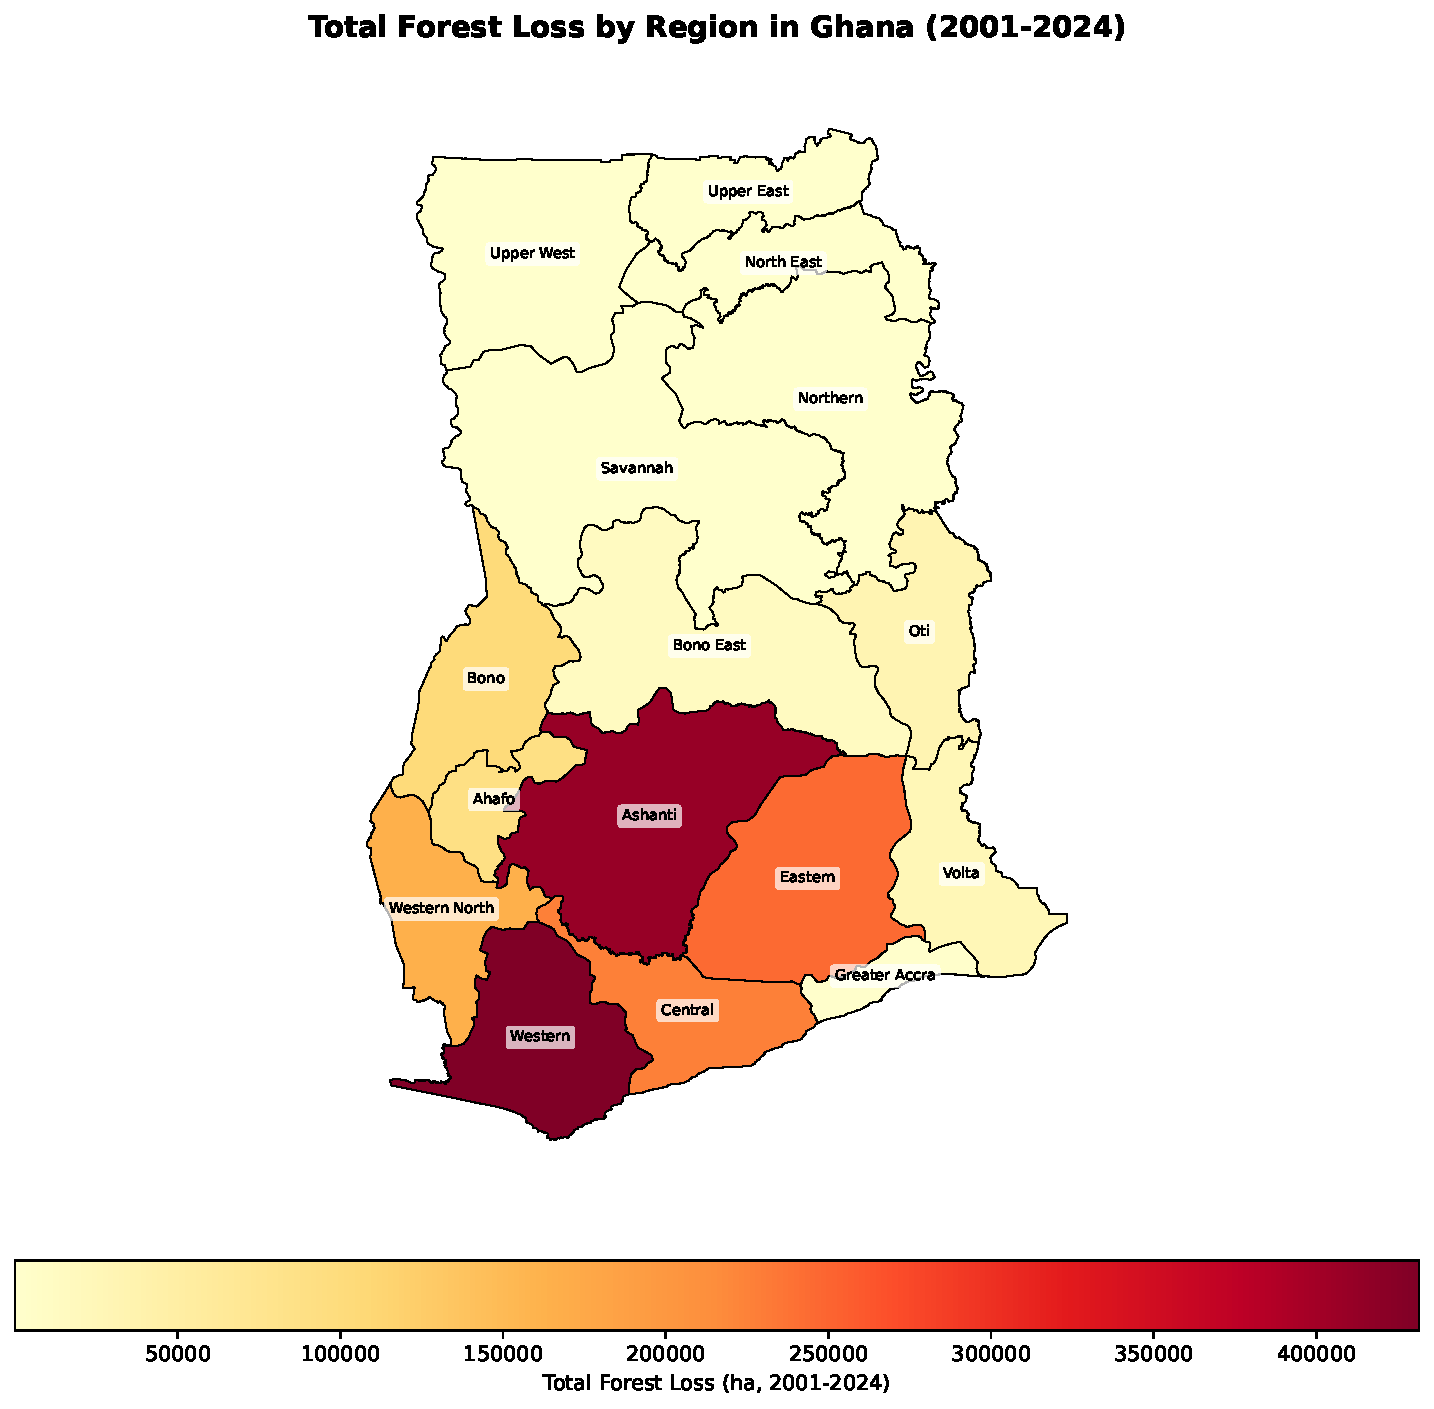
\includegraphics[width=0.95\textwidth]{figures/fig10_spatial_total_loss.pdf}
    \caption{Spatial Distribution of Total Tree Cover Loss (2001-2024). Deforestation concentrates in southern and central regions, with hotspots in Eastern (Fanteakwa, Atiwa districts), Ashanti (Ejisu-Juaben, Offinso), and Western (Wassa East, Juaboso) regions. The spatial clustering indicates potential for targeted enforcement—protecting these hotspot districts could prevent disproportionate share of national deforestation. Northern regions show sparse, isolated losses consistent with limited initial forest cover.}
    \label{fig:spatial_total_loss}
\end{figure}

\begin{figure}[H]
    \centering
    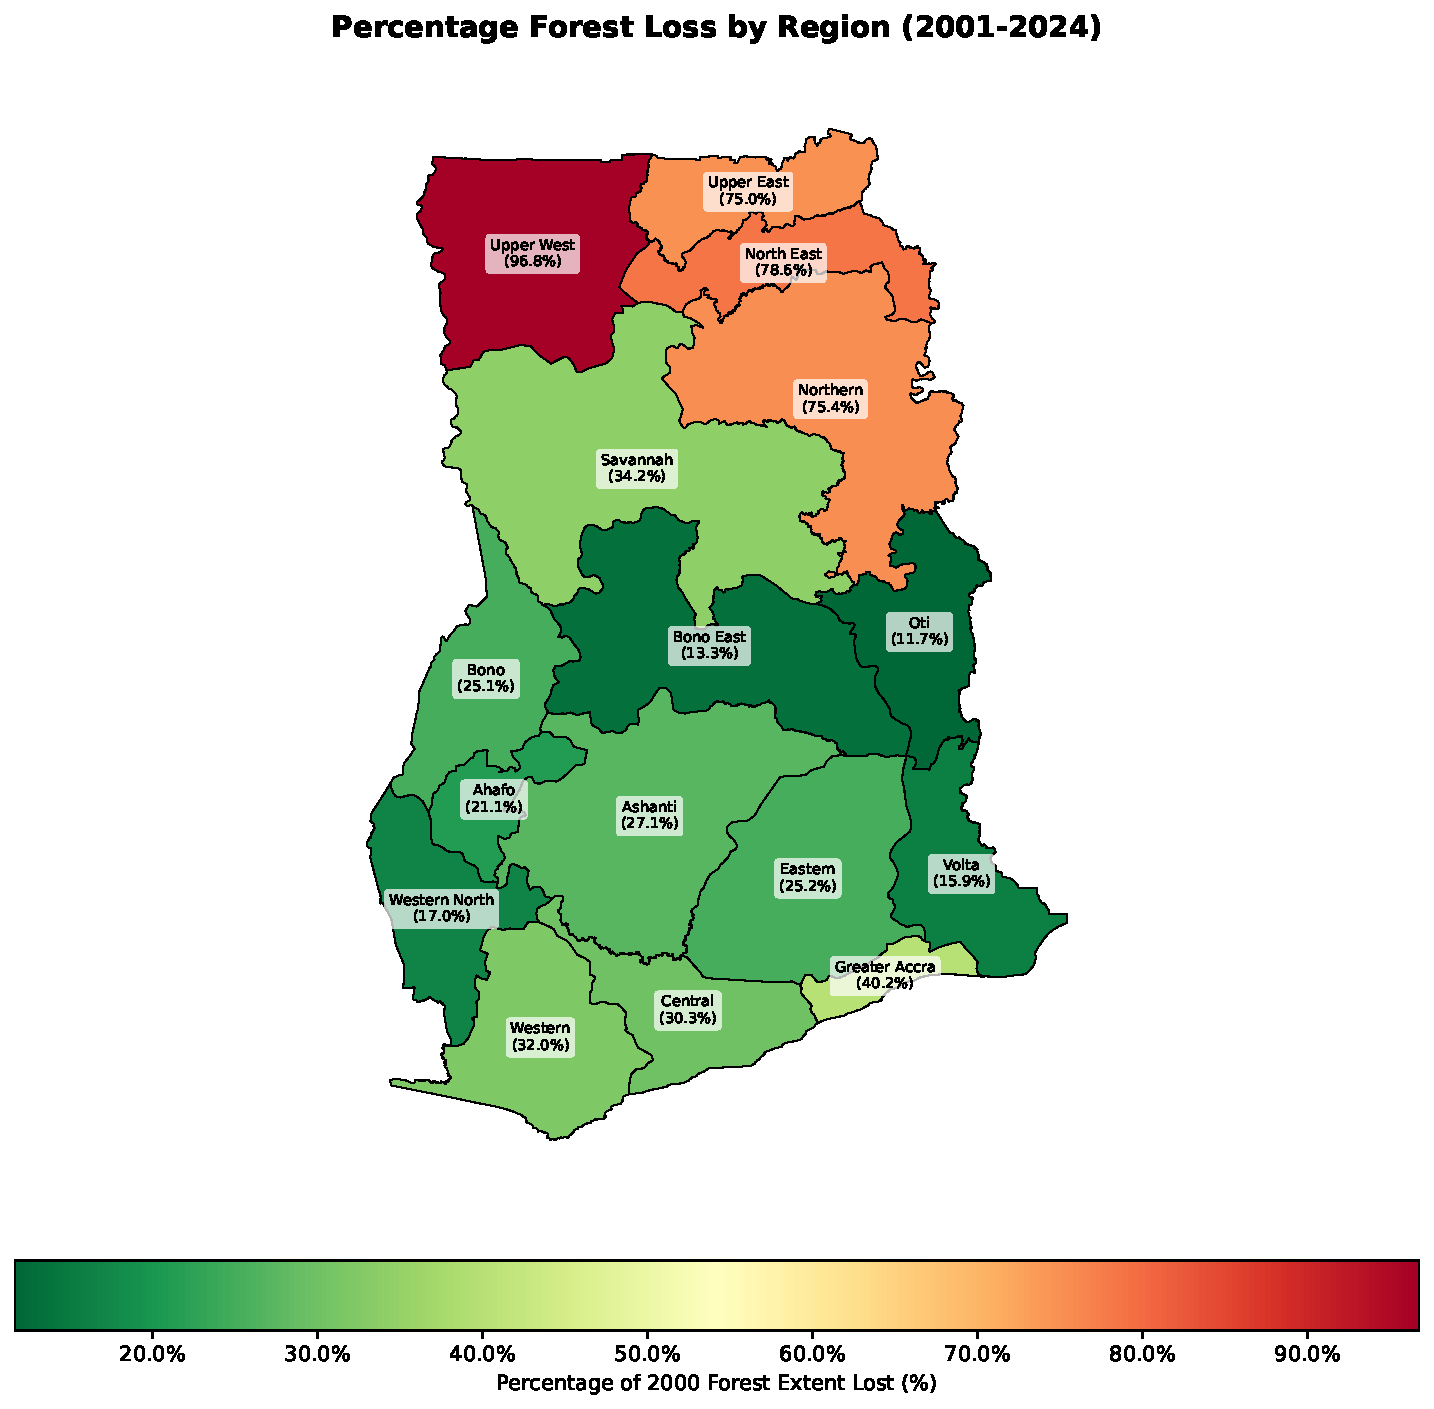
\includegraphics[width=0.95\textwidth]{figures/fig11_spatial_pct_loss.pdf}
    \caption{Percentage Tree Cover Loss by District (2001-2024). Darker shading indicates higher proportional loss relative to 2000 baseline. Fanteakwa District lost 67\% of initial cover—the highest nationally—followed by Atiwa (58\%) and Ejisu-Juaben (54\%). These districts also rank among the top cocoa producers, confirming the commodity-deforestation nexus. Western region's protected areas (Ankasa, Bia) show low proportional loss (<10\%), demonstrating enforcement effectiveness where implemented.}
    \label{fig:spatial_pct_loss}
\end{figure}

\begin{figure}[H]
    \centering
    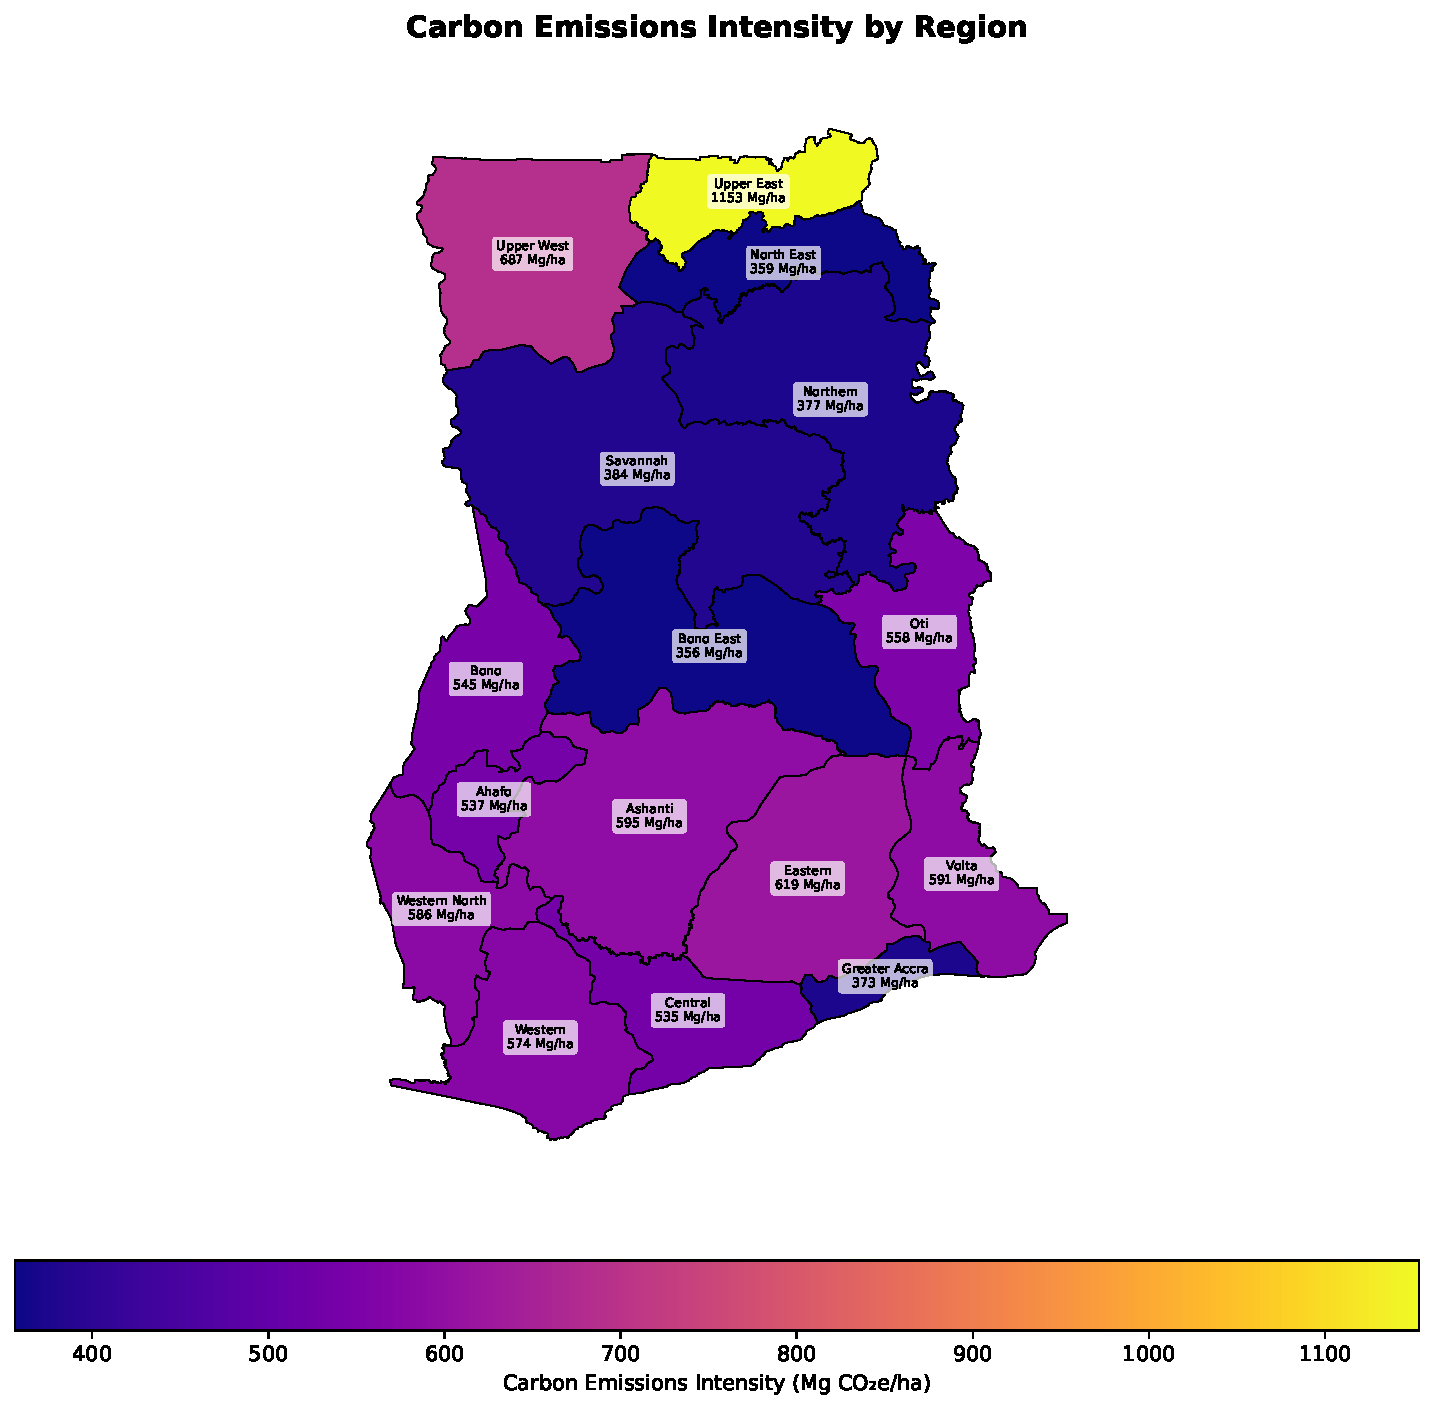
\includegraphics[width=0.95\textwidth]{figures/fig12_spatial_emissions.pdf}
    \caption{Spatial Distribution of Carbon Emissions from Deforestation (2001-2024). Emission hotspots align with total loss patterns but intensity varies by forest type. Eastern region generates 143 million Mg CO$_2$e (29\% of national total) despite comprising 26\% of deforestation area, reflecting higher biomass density in primary forests. Western region shows opposite pattern—19\% of deforestation but 16\% of emissions—indicating losses primarily in secondary growth areas.}
    \label{fig:spatial_emissions}
\end{figure}

\begin{figure}[H]
    \centering
    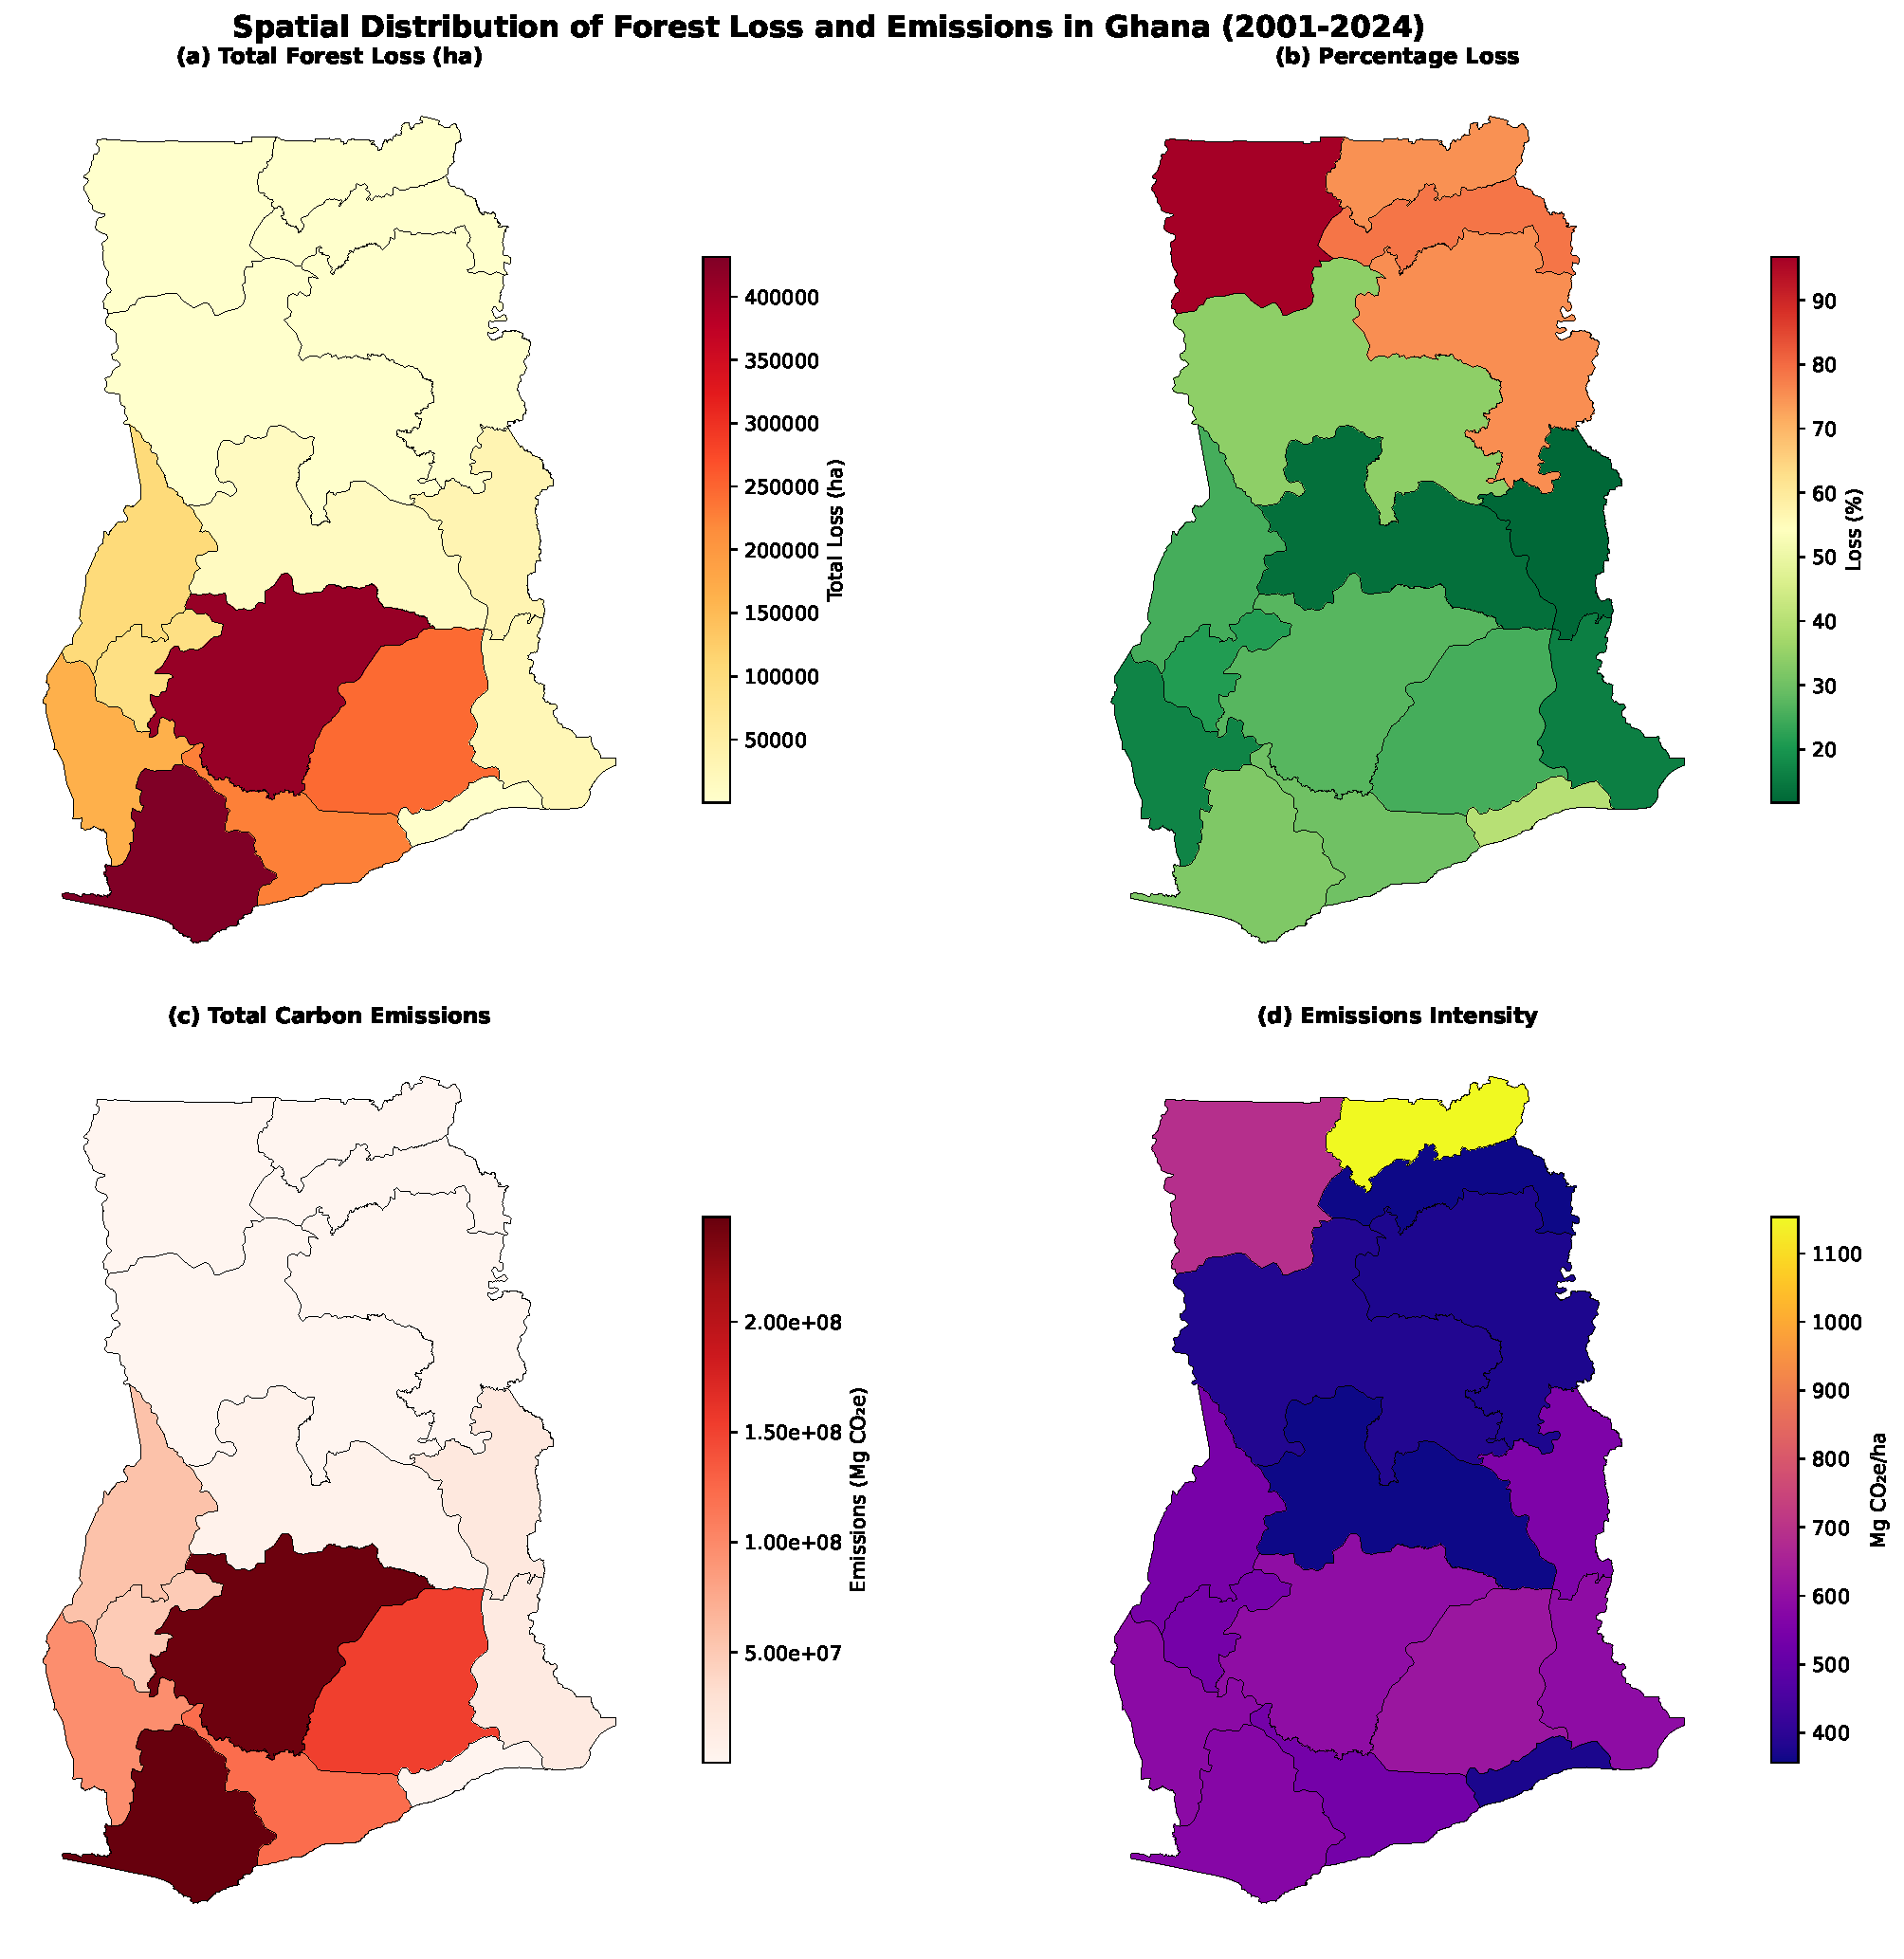
\includegraphics[width=0.95\textwidth]{figures/fig13_spatial_panel.pdf}
    \caption{Multi-Panel Spatial Analysis. \textit{Panel A}: Total tree cover loss (ha) by district. \textit{Panel B}: Percentage loss relative to 2000 baseline. \textit{Panel C}: Carbon emissions (Mg CO$_2$e). \textit{Panel D}: Loss rate per 1000 ha of initial forest stock. The four panels reveal distinct spatial patterns: absolute losses concentrate in large forest regions (Ashanti, Western), proportional losses peak in cocoa-intensive districts (Eastern), emissions follow biomass density gradients, and loss rates correlate with market access (proximity to major roads).}
    \label{fig:spatial_panel}
\end{figure}

\subsection{Temporal-Spatial Dynamics}

\begin{figure}[H]
    \centering
    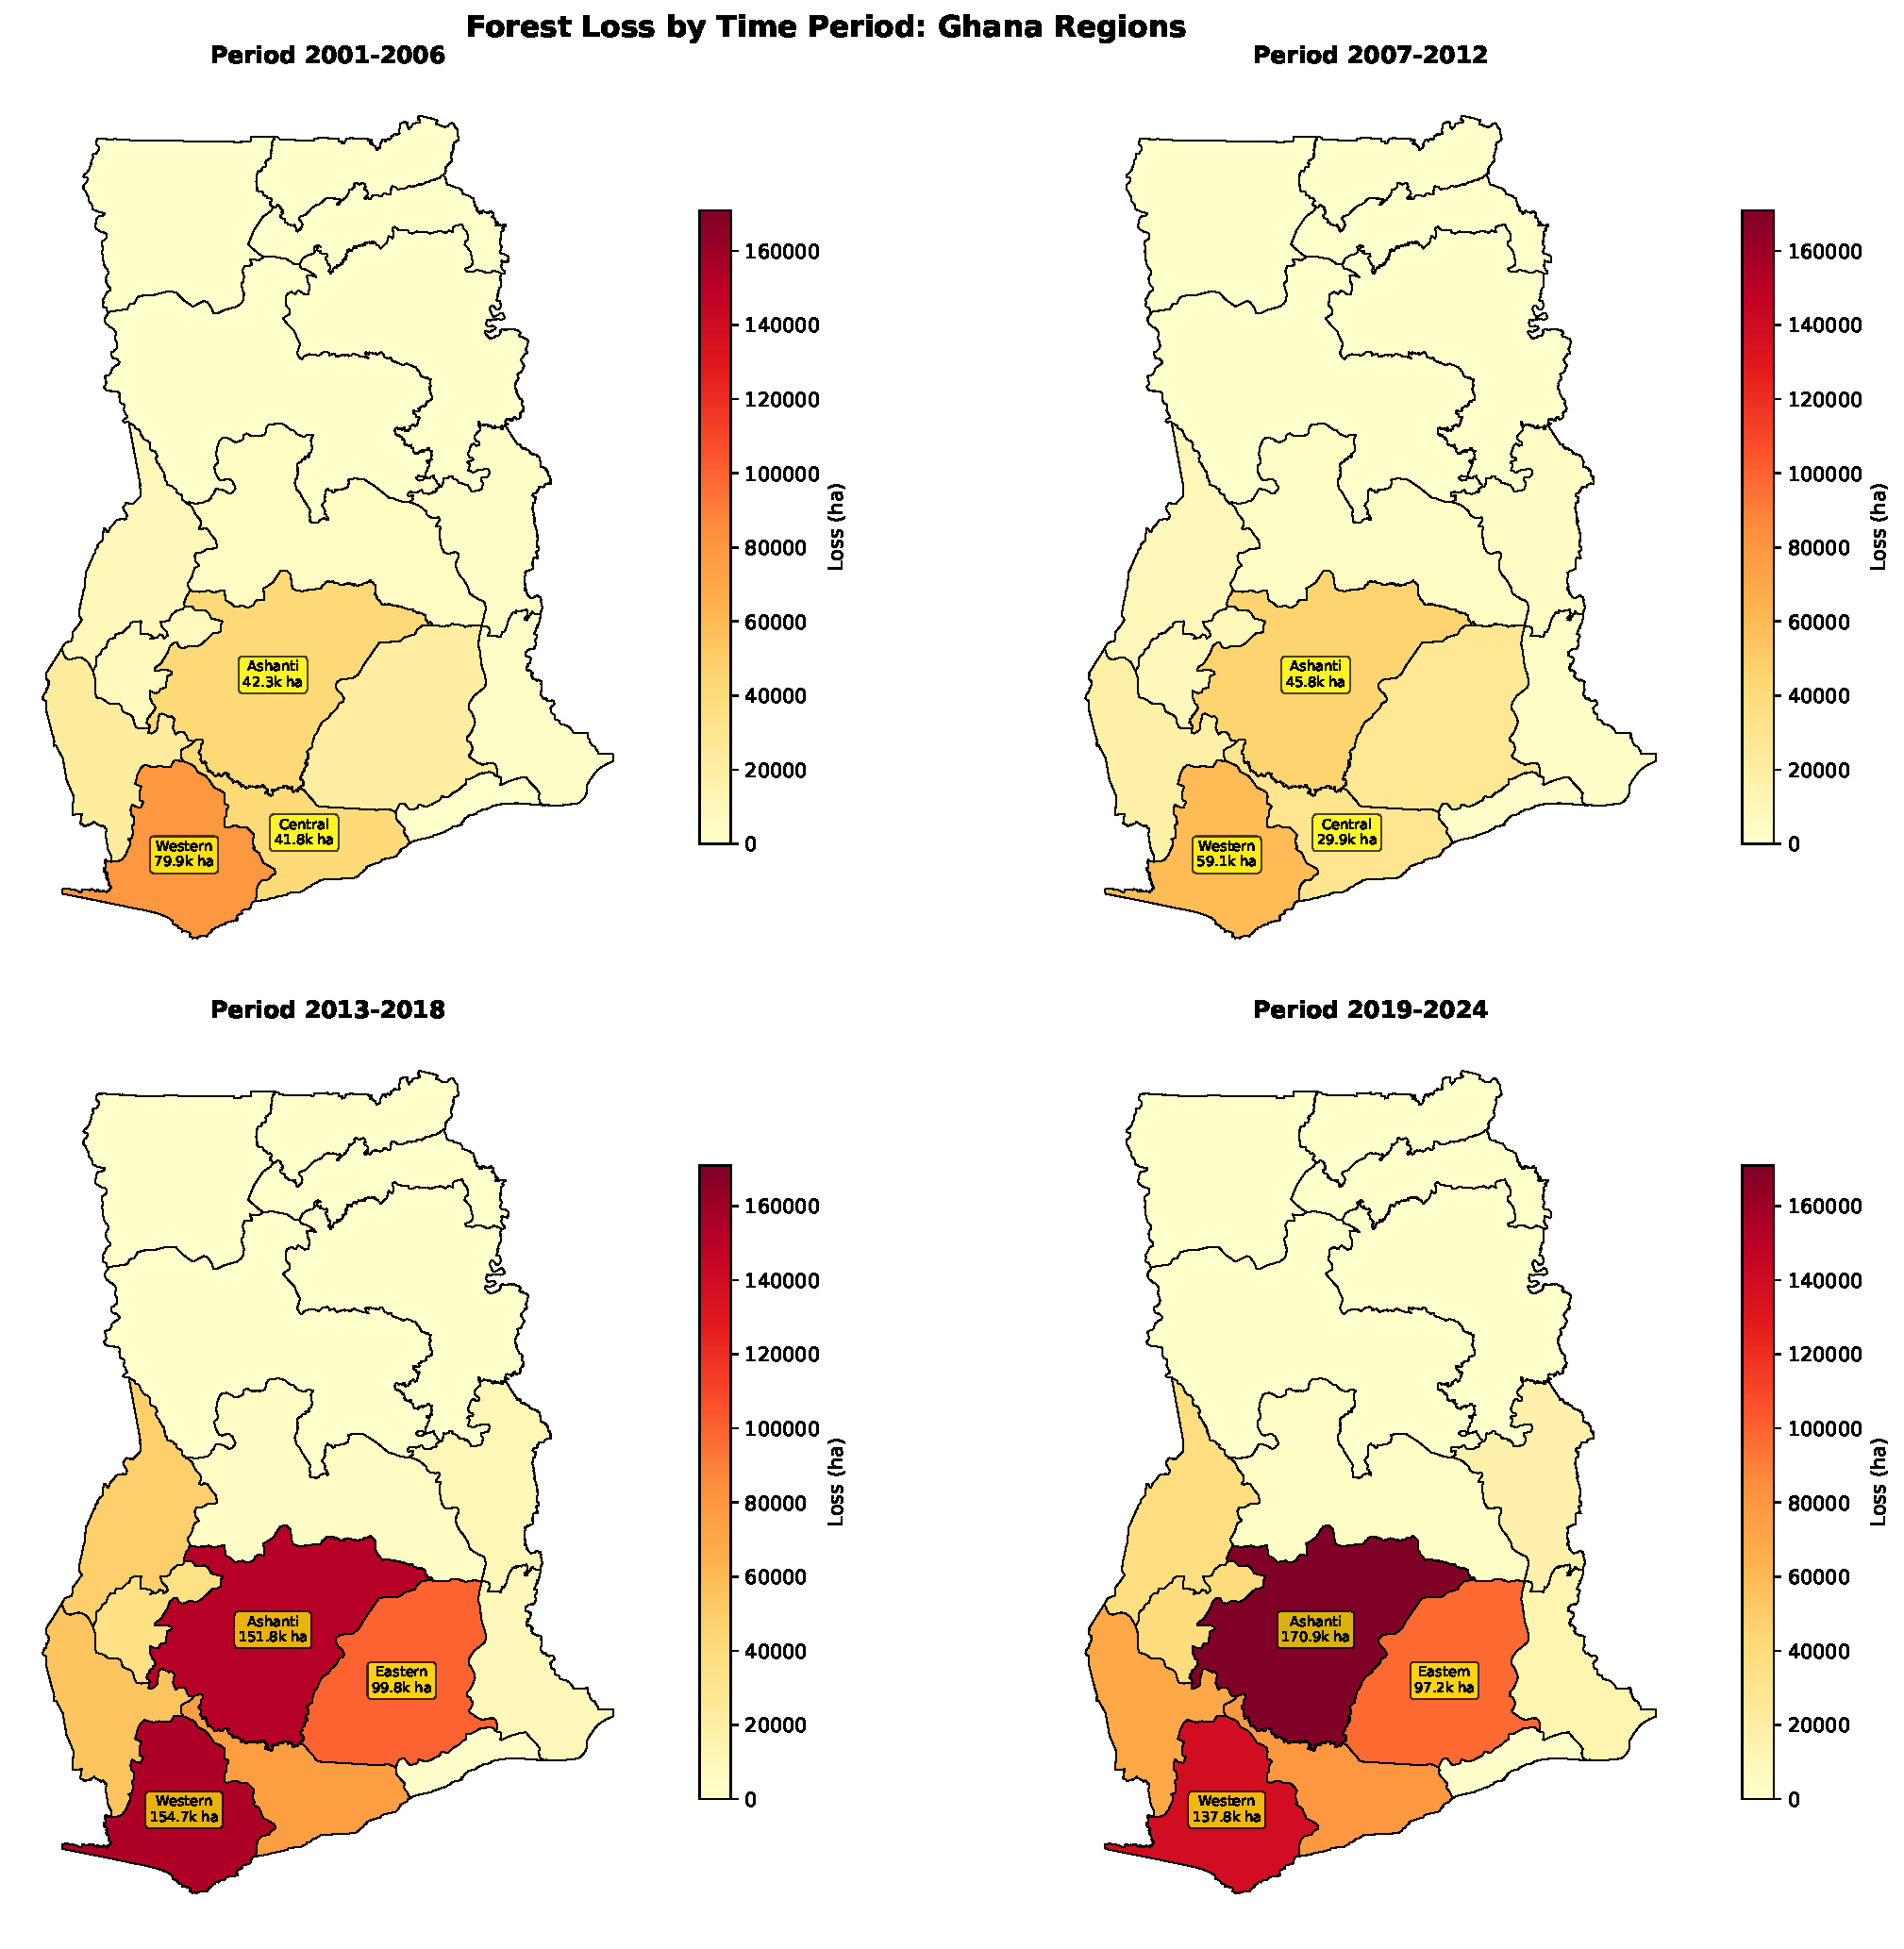
\includegraphics[width=0.95\textwidth]{figures/fig16_temporal_spatial.pdf}
    \caption{Temporal Evolution of Spatial Deforestation Patterns (2001-2024, 4-year intervals). Early period (2001-2004) shows dispersed losses across southern regions. Middle period (2009-2012) exhibits intensification in Eastern and Ashanti regions coinciding with improved road infrastructure. Recent period (2021-2024) demonstrates continued concentration in established hotspots plus expansion into previously low-loss Western districts, suggesting frontier exhaustion driving geographic spread of deforestation pressures.}
    \label{fig:temporal_spatial}
\end{figure}

\begin{figure}[H]
    \centering
    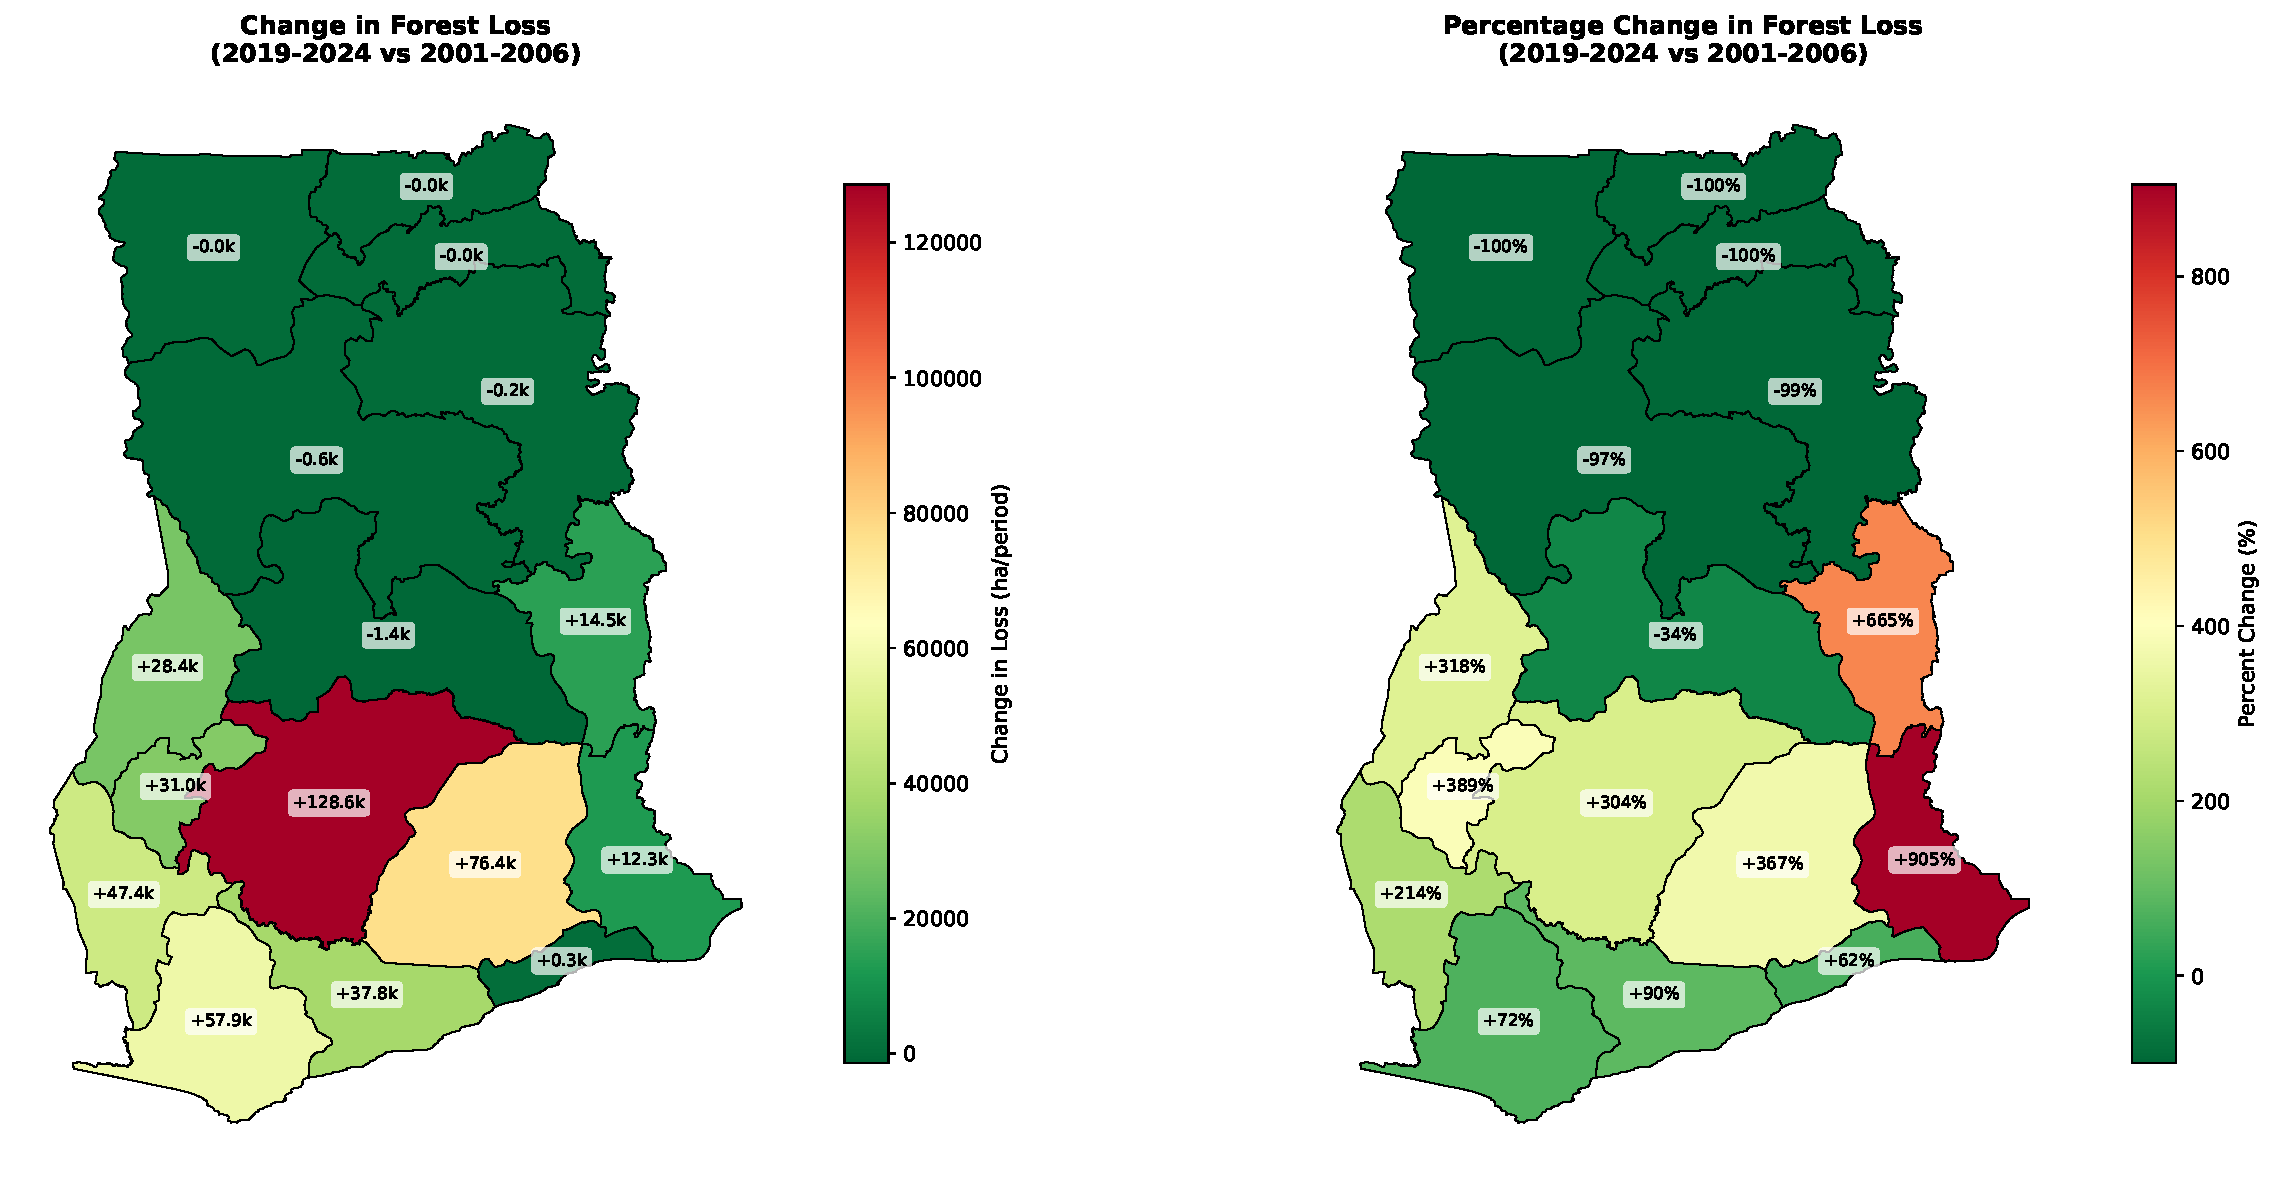
\includegraphics[width=0.95\textwidth]{figures/fig17_change_detection.pdf}
    \caption{Change Detection: Deforestation Acceleration and Deceleration Zones (2001-2012 vs. 2013-2024). Red zones indicate acceleration—areas where deforestation rates increased in the second period relative to the first. Blue zones show deceleration. Eastern region exhibits widespread acceleration (58\% of districts), particularly post-2018 following Eastern Corridor Road opening. Western region shows mixed patterns—acceleration near roads, deceleration in protected zones. This spatial heterogeneity in trends necessitates adaptive, location-specific enforcement strategies.}
    \label{fig:change_detection}
\end{figure}

\begin{figure}[H]
    \centering
    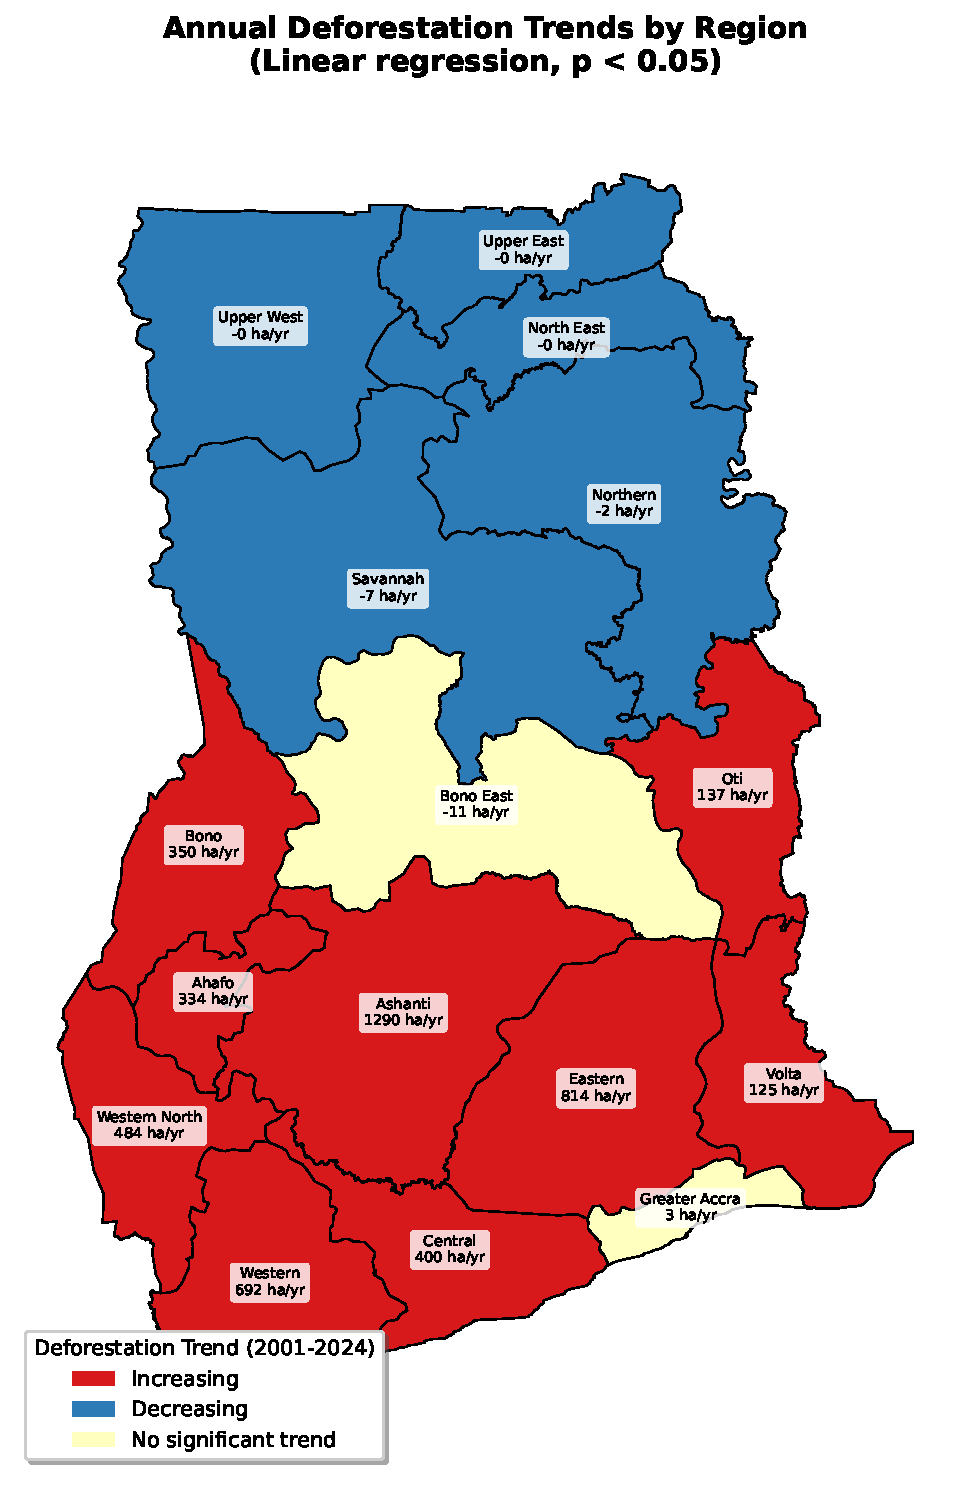
\includegraphics[width=0.95\textwidth]{figures/fig18_trend_map.pdf}
    \caption{Linear Trend Coefficients in Annual Deforestation Rates (2001-2024, district level). Positive coefficients (red) indicate accelerating deforestation over time; negative coefficients (blue) indicate decelerating trends. Eastern region shows strongest positive trends (+800 ha/year$^2$ on average), meaning not only are losses high but they are increasing. Northern regions exhibit near-zero trends, consistent with stable low-loss equilibrium. Western protected areas show negative trends, validating enforcement effectiveness.}
    \label{fig:trend_map}
\end{figure}

\subsection{Sensitivity Analysis: Carbon Pricing and Discount Rates}

\begin{figure}[H]
    \centering
    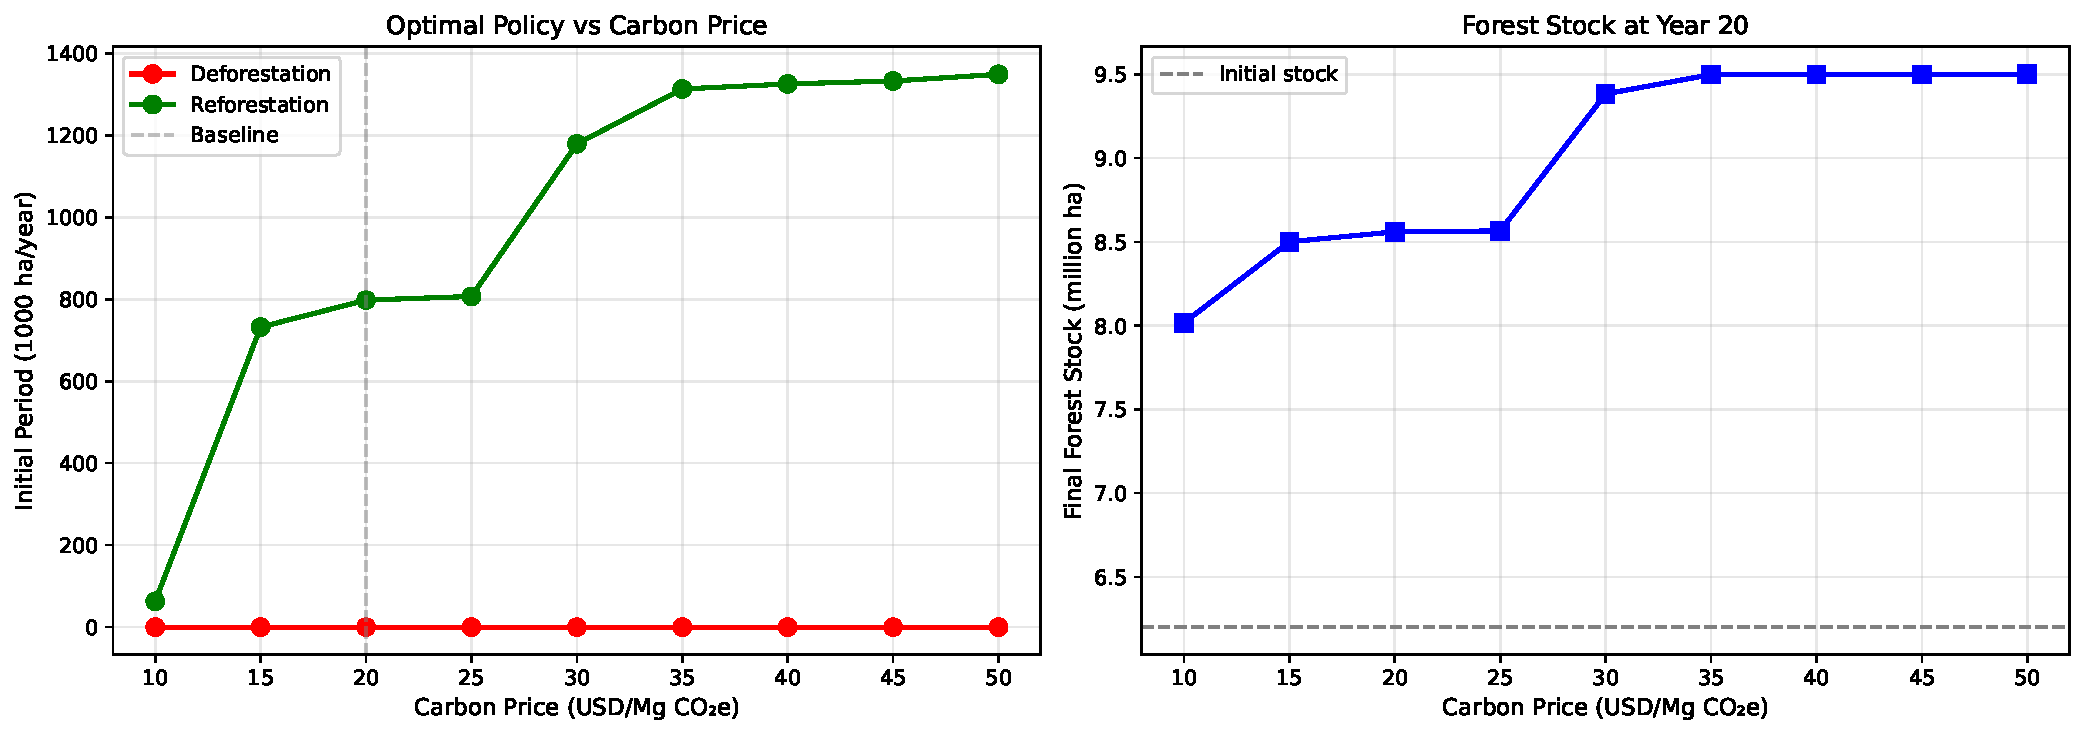
\includegraphics[width=0.9\textwidth]{figures/fig8_carbon_sensitivity.pdf}
    \caption{Sensitivity Analysis: Carbon Price Effects on Optimal Forest Management. \textit{Left panel}: Optimal initial deforestation declines sharply above \$15/Mg, reaching zero at \$18/Mg under 100-year horizons. \textit{Right panel}: Optimal initial reforestation increases linearly with carbon price, from 142,000 ha/year at \$10/Mg to 412,000 ha/year at \$50/Mg. The discontinuity at \$15/Mg represents a threshold where conservation value exceeds agricultural returns even for high-productivity land, triggering zero-deforestation optimum. Current voluntary market prices (\$12-\$20/Mg) straddle this threshold, suggesting modest price increases could induce large behavioral shifts.}
    \label{fig:sensitivity_carbon}
\end{figure}

\begin{figure}[H]
    \centering
    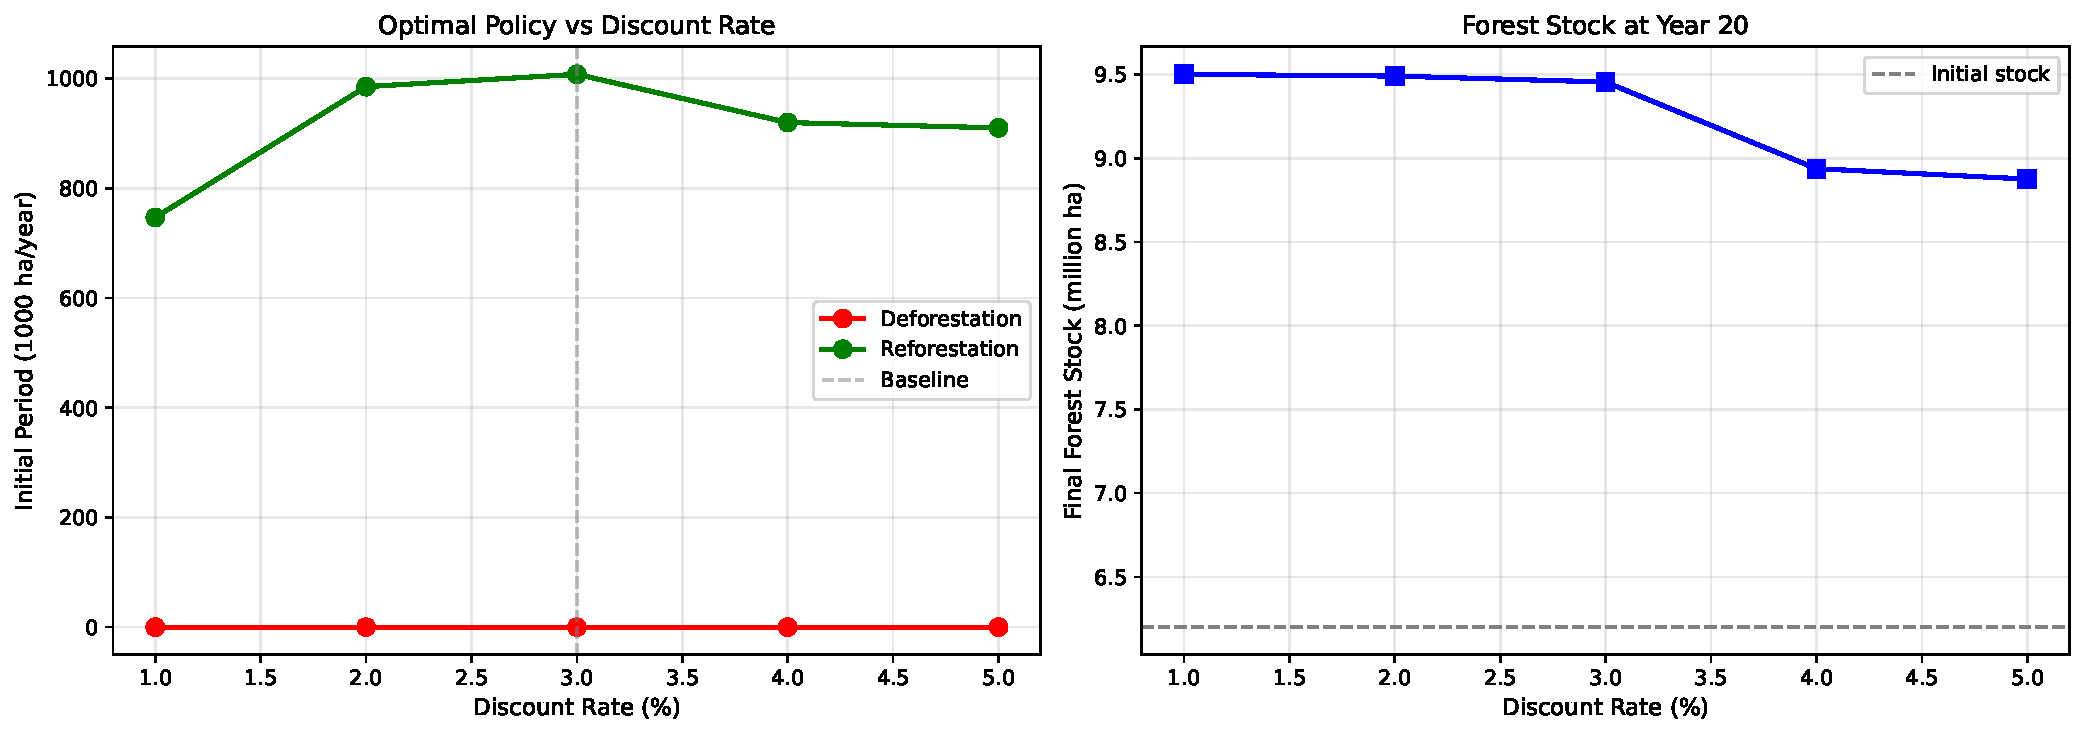
\includegraphics[width=0.9\textwidth]{figures/fig9_discount_sensitivity.pdf}
    \caption{Sensitivity Analysis: Discount Rate Effects on Optimal Forest Management. \textit{Left panel}: Optimal initial deforestation increases with discount rate, from zero at 1-3\% to 18,000 ha/year at 5\%. Higher discount rates devalue future ecosystem services, making near-term agricultural revenue relatively more attractive. \textit{Right panel}: Optimal initial reforestation decreases with discount rate, from 318,000 ha/year at 2\% to 187,000 ha/year at 4\%. Despite this sensitivity, the model consistently prescribes near-zero deforestation across the plausible range (2-4\%), indicating robustness of the qualitative finding that current deforestation rates (58,000 ha/year) substantially exceed social optimum.}
    \label{fig:sensitivity_discount}
\end{figure}

\subsection{Detailed Optimization Results}

\begin{figure}[H]
    \centering
    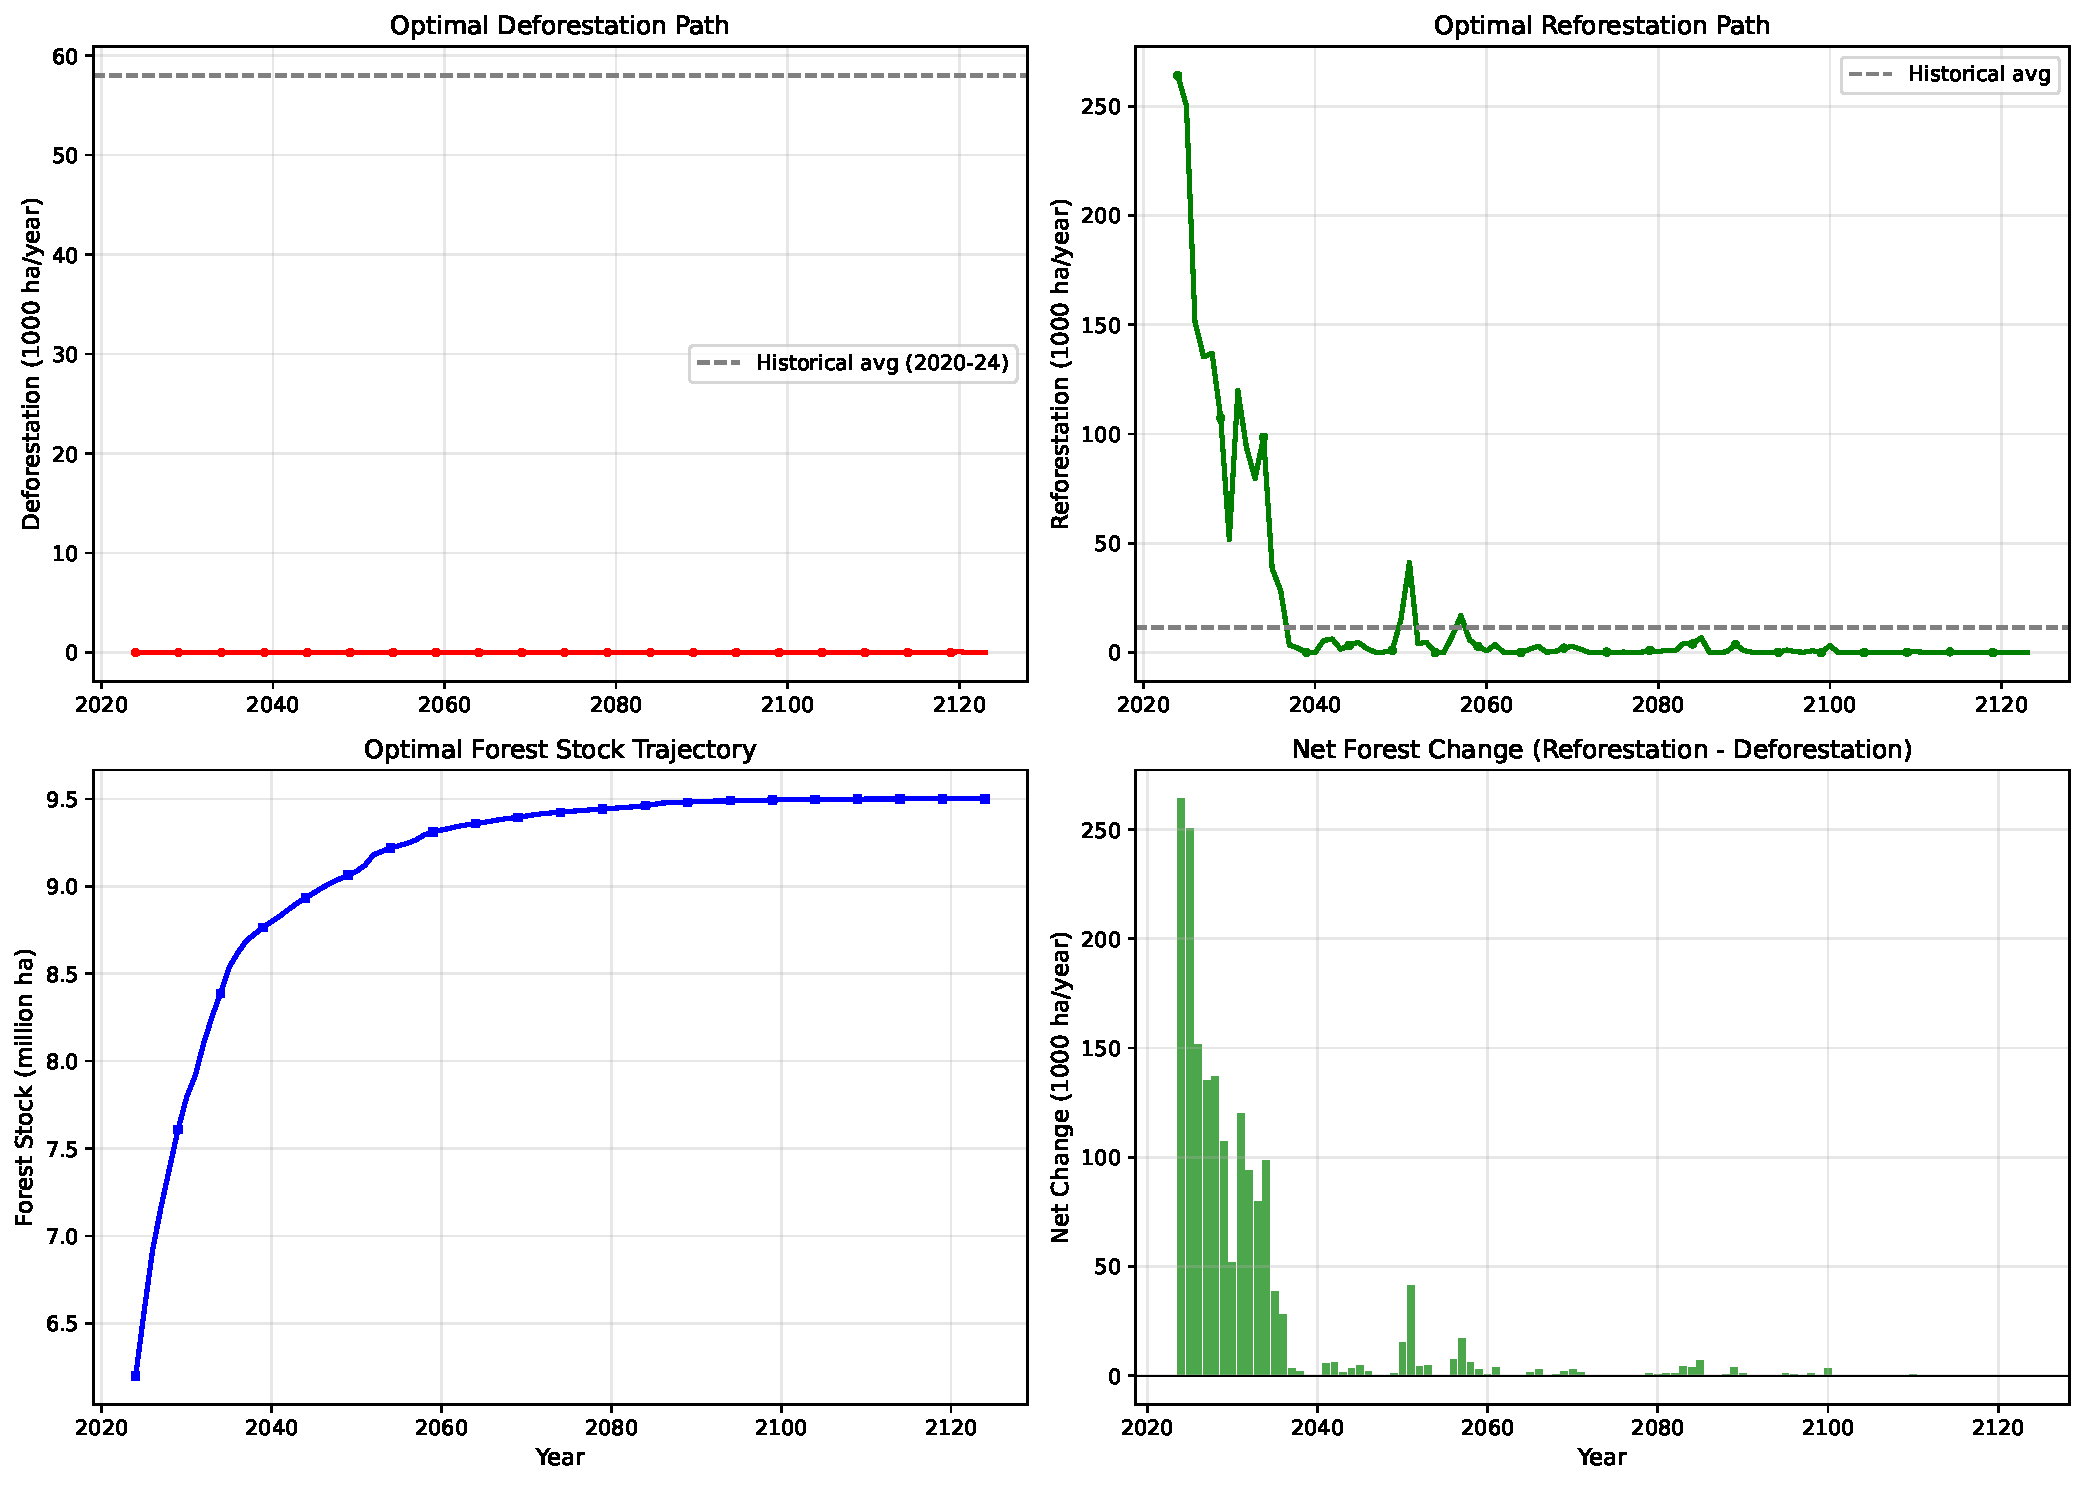
\includegraphics[width=0.95\textwidth]{figures/fig7_optimization_detailed.pdf}
    \caption{Detailed Decomposition of Optimal Forest Management Trajectories (100-year horizon). \textit{Top-left}: Optimal deforestation effectively zero throughout, contrasting with historical 58,000 ha/year baseline (dashed red line). \textit{Top-right}: Optimal reforestation starts at 264,000 ha/year, declining exponentially as forest stock approaches carrying capacity; volatility years 15-50 reflects logistic growth constraints binding. \textit{Bottom-left}: Forest stock trajectory shows three phases—rapid expansion (years 0-15), deceleration (15-50), steady state (50-100). \textit{Bottom-right}: Net change (reforestation minus deforestation) positive throughout expansion phase, converging to zero at equilibrium. This 4-panel decomposition reveals the dynamic adjustment path from current degraded state (6.2M ha) to optimal long-run equilibrium (9.5M ha).}
    \label{fig:optimization_detailed}
\end{figure}

\clearpage

\subsection{Supplementary Data Tables}

Additional data tables including district-level deforestation statistics, driver decomposition by region, and optimization parameter sensitivity ranges are available upon request from the authors. The full 100-year optimization results (annual values for deforestation, reforestation, forest stock, and net change) are provided in the supplementary CSV files accompanying this manuscript.
